\chapter{Experiment}\label{Experiment}

Nu we in alle achterliggende theorie in hoofdstuk \ref{Lectuur} gezien hebben, kunnen we van start gaan met het experiment. Het doel van het experiment is aan de hand van enkele algemene technieken uit te Machine Learning een gevoelsanalyse te kunnen uitvoeren op Nederlandse tekst waarbij we een algoritme het onderscheidt willen tussen positief negatief. Zodanig wanneer we het algoritme een onbekende tekst geven, het kan bepalen of de tekst een positieve of negatieve emotie uitdrukt. De prestatie van zo'n algoritme wordt in dit experiment beoordeeld op basis van de classificatieprecisie.  Wanneer het algoritme met een hoge precisie classificeert en bijna alles input correct kan classificeren als positief of negatief, dan spreken we van een goede prestatie. Wanneer de classificatieprecisie rond de 50\% of minder ligt, spreekt men van een slechte prestatie. Een classificatieprecisie van 50\% kan men vergelijken met een classificatiealgoritme dat telkens bij het bepalen van de output een munt gaat opgooien en op basis van kop of munt de output bepalen. Wat neerkomt op het random bepalen van de output.\\
%
Vooraleerst we aan het de resultaten van het experiment bekijken, hebben we het in \ref{De Dataset} over de dataset die we gebruiken. Er is gekozen om gevoelsanalyse uit te voeren op film-, boek- en muziekrecensies  en in deze sectie wordt uitgelegd waarom en hoe het verzamelen van de data is verlopen. In \ref{Naive Bayes Classifier met verschillend onderwerp voor trainings- en testset} en \ref{Naive Bayes Classifier met hetzelfde onderwerp voor trainings- en testset} volgen dan de experimenten en als laatste vatten we alle de bevindingen van het experiment samen in \ref{Conclusie experiment}.

\section{De Datatset}\label{De Dataset}

Zoals in de introductie staat vermeld waren film- ,boek- en muziekrecensies niet de eerste keuze. Eerst was het idee om de data van sociale media te nemen zoals tweets van Twitter. Er zou dan rond een bepaald onderwerp tweets verzamelen zoals bijvoorbeeld de nieuwe treinregeling van de NMBS. Omdat we voor het experiment gebruik maken van supervised learning technieken moesten we de tweets manueel labelen als positief of negatief om de tweets als trainingsset te kunnen gebruiken. Naast het feit dat het manueel labelen van de tweets een relatief intensief werkje is, werd er ook opgemerkt dat er veel sarcasme heerst op Twitter. Voor bepaalde mensen is het al moeilijk voor sarcasme te herkennen en voor een algoritme is het dat zeker. Sarcastische tweets zijn onbruik voor de training van de algoritmen en zorgen voor ruis in de dataset. De oplossing lag dan bij film-, muziek- en boekrecensies. Recensies bieden alles wat we nodig hebben. Een recensie is of te wel positief, negatief of neutraal. Maar doordat er meestal een rating aanwezig bij de review is het gemakkelijk om automatische te labelen en enkel de positieve en negatieve reviews op te nemen in onze dataset. De keuze om recensies te nemen over films, boeken en muziek was een beredeneerde keuze. Het aanbod is enorm, meestal niet te specifiek en toegankelijk. Merk op bij het verzamelen van de recensies gefocust werd op korte recensies van gebruikers en niet op de uitgebreide recensies van dagbladen. De recensies voor dit experiment zijn afkomstig van moviemeter.nl, boekmeter.nl en muziekmeter.nl. Deze websites waren de perfecte bron aan informatie. Ze bevatten allemaal toplijsten met films, boeken of muziekalbums waarop vele gebruikers hun persoonlijke mening plaatsen. Samen met die mening laten ze telkens ook een score op 5 achter, die het gevoel bij het betreffende item weerspiegeld. Perfect dus om de labeling van de meningen te automatiseren en een duidelijk onderscheidt te maken tussen positieve en negatieve meningen. Voor dataset van het experimenten werden recensies met een score lager of gelijk aan twee op vijf beschouwd als negatief en recensies met een score gelijk of groter dan drie op vijf beschouwd als positief.\\

\begin{figure}[h]%
    \centering
    \subfloat{{
\includegraphics[width=10cm]{voorbeeldrecensie} }}%
    \caption{Een voorbeeld van een positive commentaar op \url{moviemeter.nl}}%
\end{figure}

 Alle recensies zijn afkomstig van de ``All Time Top 250''-toplijst op de betreffende website. Door deze lijsten waren we zeker dat voldoende recensies aanwezig waren. Onderstaande tabel geeft het aantal verzamelde recensies van ieder onderwerp weer, waarbij een onderscheidt wordt gemaakt tussen positief en negatief.

\begin{table}[h]
\centering
\begin{tabular}{l|l|l|l|}
\cline{2-4}
                                        & \textbf{Films} & \textbf{Muziek} & \textbf{Boeken} \\ \hline
\multicolumn{1}{|l|}{\textbf{Positief}} & 197358         & 15197           & 146             \\ \hline
\multicolumn{1}{|l|}{\textbf{Negatief}} & 17978          & 3019            & 3719            \\ \hline
\end{tabular}
\caption{Aantal verzamelende recensies} 
\end{table}

Wat meteen opvalt is dat er aanzienlijk minder positieve boekrecensies verzameld zijn. Hier zullen we rekening mee moeten houden tijdens het experiment. Voor de andere categorie\"en zijn de positieve recensies in grote aantallen aanwezig, wat waarschijnlijk te maken heeft met dat we de ``All Time Top 250''-toplijst gebruiken als databron.

\begin{figure}%
    \centering
    \subfloat{{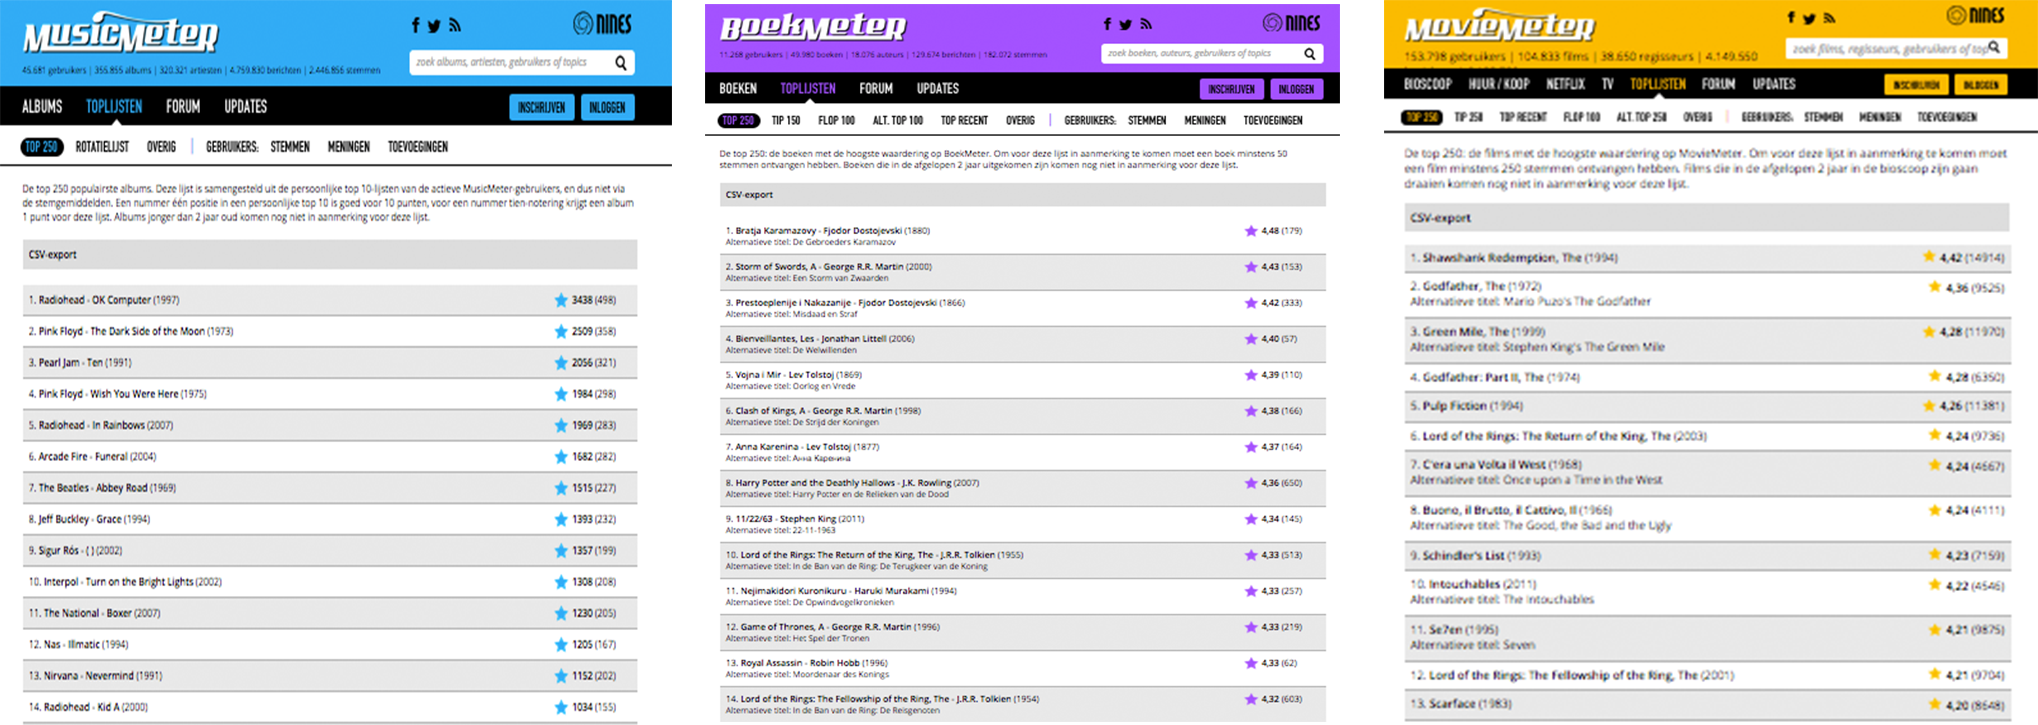
\includegraphics[width=15cm]{toplijsten} }}%
    \caption{de ``All Time Top 250''-toplijsten op de websites}%
\end{figure}

\section{Naive Bayes Classifier met hetzelfde onderwerp voor trainings- en testset}\label{Naive Bayes Classifier met hetzelfde onderwerp voor trainings- en testset}

Als eerste experiment gaan we kijken hoe de prestaties van de classifier zijn bij het trainen en testen met data van dezelfde soort. Bijvoorbeeld we trainen met een trainingsset van filmrecensies en testen het getrainde algoritme op een testset van filmrecensies. Dit gaan we voor zowel films, boeken als muziek doen. Als classifier nemen we de Naive Bayes Classifier, in sectie \res{Naive Bayes Classifier} zeiden we al dat dit een goede eerste keuze is als leermethode. Verder geven de data mee aan de classifier als een Bag of Words met TFIDF weging\\
%
Algemeen voor alle experimenten zijn de resultaten berekend als gemiddelde over dertig runs. Dit wil zeggen dat er telkens bij iedere run een nieuwe Naive Bayes Classifier wordt aangemaakt,getraind en getest wordt met een andere trainings- en testset als de andere runs. Na het uitvoeren van die runs wordt hier dan het gemiddelde van genomen. Verder worden het aantal benodigde trainings- testsamples random geselecteerd uit onze grote pool van recensies. Verder bestaan de resultaten van experimenten uit de classificatieprecisie van zowel de trainings- en testset, een confidence interval voor 95\%, de standaard afwijking en de confusion matrix. Een confusion matrix geeft aan hoeveel van elke outputmogelijkheden er juist zijn ge\"identificeert door de classifier en hoeveel er fout als juist zijn ge\"indentificeerd, ook wel valse positieve genoemd. Als laatste wordt er ook de learningcurve bekeken om over- of underfitting uit te sluiten.


\renewcommand\arraystretch{1.5}
\setlength\tabcolsep{0pt}
\begin{table}[h]
\centering
\begin{tabular}{c >{\bfseries}r @{\hspace{0.7em}}c @{\hspace{0.4em}}c @{\hspace{0.7em}}l}
  \multirow{10}{*}{\parbox{1.1cm}{\bfseries\raggedleft eigelijke\\ waarden}} & 
    & \multicolumn{2}{c}{\bfseries output voorspelling} & \\
  & & \bfseries p & \bfseries n  \\
  & p$'$ & \MyBox{Waar}{Positief} & \MyBox{Vals}{Negatief}  \\[2.4em]
  & n$'$ & \MyBox{Vals}{Positief} & \MyBox{Waar}{Negatief} \\
\end{tabular}
\caption{Illustratie van de confusion matrix} 
\end{table}


\subsection{Films als trainings- en testset}\label{Films als trainings- en testset}

Eerst trainen en testen we de Naive Bayes Classifier met filmrecensies. De trainingsset bestaat uit 6000 samples en de testset uit 2000 samples. Zoals eerder vermeld werden deze samples random geselecteerd en is het volgende resultaat het gemiddelde van 30 runs.\\
\newline
\textbf{Standaard afwijking} = 0.0094\\
\textbf{95\% Confidene Interval} = (0.70656666666666668, 0.70300502660338759, 0.71012830672994576)\\
 
\begin{table}[h]
\centering
\setlength\tabcolsep{4pt}
\begin{minipage}{0.48\textwidth}
\centering
\begin{tabular}{l|l|}
\cline{2-2}
                                            & \textbf{Precisie} \\ \hline
\multicolumn{1}{|l|}{\textbf{Trainingsset}} & 90,52\%           \\ \hline
\multicolumn{1}{|l|}{\textbf{Testset}}      & 70,66\%           \\ \hline
\end{tabular}
\caption{Precisie Naive Bayes Classifier getraind op filmrecensies}
\label{tab:accuracy}
\end{minipage}%
\hfill
\begin{minipage}{0.48\textwidth}
\centering
\begin{tabular}{lll}
                                 & \textbf{P}               & \textbf{N}               \\ \cline{2-3} 
\multicolumn{1}{l|}{\textbf{P'}} & \multicolumn{1}{l|}{824} & \multicolumn{1}{l|}{175} \\ \cline{2-3} 
\multicolumn{1}{l|}{\textbf{N'}} & \multicolumn{1}{l|}{410} & \multicolumn{1}{l|}{589} \\ \cline{2-3} 
\end{tabular}
\caption{Confusion matrix testset Naive Bayes Classifier, getraind met filmrecensies} 
\label{tab:ompdiff} 
\end{minipage}
\end{table}




\subsection{Muziek als trainings- en testset}\label{Muziek als trainings- en testset}

Nu trainen en testen we de Naive Bayes Classifier met muziekrecensie. De trainingsset bestaat uit 6000 samples en de testset uit 2000 samples. Wederom werden deze samples random geselecteerd en is het volgende resultaat het gemiddelde van 30 runs.


\subsection{Boeken als trainings- en testset}\label{Boeken als trainings- en testset}

Als laatste trainen en testen we de Naive Bayes Classifier met boekrecensies. De trainingsset bestaat uit 6000 samples en de testset uit 2000 samples. De samples zijn wederom random geselecteerd en het resultaat is het gemiddelde van 30 runs.



\section{Naive Bayes Classifier met verschillende onderwerp voor trainings- en testset}\label{Naive Bayes Classifier met verschillend onderwerp voor trainings- en testset}

\subsection{Films als trainings- en testset}\label{Films als trainingsset}
\subsubsection{Muziek als testset}\label{Muziek als testset}
\subsubsection{Boeken als testset}\label{Boeken testset}
\subsection{Muziek als trainings- en testset}\label{Muziek als trainingsset}
\subsubsection{Films als testset}\label{Films als testset}
\subsubsection{Boeken als testset}\label{Boeken testset}
\subsection{Boeken als trainings- en testset}\label{Boeken als trainings- en testset}
\subsubsection{Films als testset}\label{Films als testset}
\subsubsection{Muziek als testset}\label{Muziek als testset}
\subsubsectionf{Conclusie experiment}\label{Conclusie experiment}

Als hoofddoel willen we te weten komen of het mogelijk is om met algemene technieken uit de machine learning goede classificatieresultaten kunnen behalen. Goede classificatieresultaten uit zich in de precisie waar de classifier met classificeert. In dit onderzoek gaat dit de metriek zijn waarop we bepalen of een classificatie goed of slecht verloopt.\\
We gebruiken de eerder besproken classifiers, namelijk een Naive Bayes classifier en Decission tree als zelflerende algoritmen en trainen Naive bayes classifier telkens met een ander voorbewerkte dataset. De Decission tree trainen we enkel met een LSA voorbewerkte dataset. Als laatste analyseren de telkens de resultaten op basis van de testset en de voorbewerkingstechniek die gebruikt wordt op de dataset.

\section{Resultaten}\label{Resultaten}

Belangrijk om te melden dat volgende resultaten afkomstig zijn door de classifiers te trainen met een moviedataset van 8000 samples, random gekozen, waarvan 6000 trainsamples en 2000 testsamples en dit gemiddeld genomen over 10 runs.
Merk op dat zowel de testset als trainigsset evenwichtig verdeeld zijn.  Dit wil zich dat precies de helft van de set positief is en de andere helft negatief.

Verder wordt er telkens paarsgewijs getest. De testset is altijd hetzelfde voorbewerkt als de trainingsset van de classifier.

Het eerste wat hier is weergegeven, zijn de resultaten van een Naive Bayes Classifier met als trainingsset filmrecensies en als testset film- , muziek en boekrecensies. 


Wat meteen is dat er niet echt een beduidend verschil is tussen de pre-procestechnieken. Ook zien we in tabel 3.BLA dat de beste resultaten worden behaald wanneer de train- en testset van dezelfde soort zijn. \\

Volgende classificatieresultaten komen voort uit de classificatie waarbij de train- en testresultaten telkens voorbewerkt zijn door alle stopwoorden en leestekens te verwijderen. Dan de sets om te vormen naar een tfidf-matrix en tenslotte LSA uit te voeren en ieder document te reduceren naar 2 features.
%
%resultaten lsa voor verschillende models TFIDF , verwijderen van stopwoorden, LSA 
\begin{table}[h]
\centering
\begin{tabular}{|l|l|l|}
\hline
\textbf{Model}              &\textbf{Precisie Trainingsset}    &\textbf{Precisie Testset}    \\   \hline
Decision Tree               & 99,77\%                          & 99,22\%                     \\  \hline
Naive Bayes classifier      & 99,82\%                          & 51,35\%                     \\ \hline 
\end{tabular}
\caption{Resultaten van de classifiers met als trainingsset en testset filmrecensies, beide voorbewerkt door LSA }
\end{table}

Deze resultaten zijn zeer interessant. Er is duidelijk een groot verschil tussen de precisie van de testset voor de Decision Tree en de Naive Bayes classifier. De Naive Bayes classifier kan totaal niets opmaken uit de LSA features die een document voorstellen. Zeker als je weet als men random zou sorteren de precisie 50\%  zou bedragen. Aan de andere hand zijn de resultaten van de decision tree in combinatie met de  lsa features verrassend goed. Met bij een perfecte classificatie kan de decision tree heel goed het onderscheidt maken tussen positieve en negatieve filmrecensies. Wat een veel betere prestatie is, dan de Naive bayes classifier waarbij men hoogste 64,70\% haalde.

Dit resultaat kan men niet negeren er vergt een dieper onderzoek. Wat we  voorlopig weten op basis van de resultaten is:
%
\begin{itemize}
  \item De Naive Bayes Classifier heeft in het algmeen een slechte classificatieprestatie, zowel wanneer train- en testset van dezelfde soort of verschillend zijn.
  \item De classificatie verbetert niet beduidend wanneer men een andere pre-processing techniek gebruikt.
  \item Classificatie aan de hand van LSA features in combinatie met een decision tree classifier levert goede resultaten op wanneer train- en testset van dezelfde soort zijn.
\end{itemize}
\\
Nu we dit weten, bekijken we de combinatie van LSA en de decision tree classifier wat meer in detail. In de uitdieping gaan we bekijken hoe de classificatieresultaten zich verhouden wanneer men een zelfde of verschillende train- en testset gebruikt. Verder gaan we deze resultaten met die van de Naive Bayes Classifier in dezelfde omstandigheden. Als laatste proberen we classificatieresultaten van de decision tree grafisch in kaart te brengen en te kijken waarom het niet of wel goed presteert.   


\section{Uitdieping onderzoek}\label{Deel 2}

Onderstaande tabel geeft alle classicatieresultaten weer, waarbij de kolommen het type van de trainingsset voorstelt en de rijen de testsets.

\begin{table}[h]
\centering
\setlength\tabcolsep{4pt}
\begin{minipage}{0.48\textwidth}
\centering
\begin{tabular}{|l|l|l|l|}
\hline
Testset & Movies  & Muziek  & Boeken  \\  \hline
Movies  & 98,90\% & 44,01\% & 47,56\% \\  \hline
Muziek  & 57,60\% & 98,67\% & 45,93\% \\ \hline
Boeken  & 42,83\% & 51,89\% & 94,32\% \\ \hline
\end{tabular}
\caption{Resultaten van de classificatie met een Decision Tree, getrained op LSA features met verschillende soorten trainings- en testsets}
\label{tab:accuracy}
\end{minipage}%
\hfill
\begin{minipage}{0.48\textwidth}
\centering
\begin{tabular}{|l|l|l|l|}
\hline
Testset & Movies   & Muziek & Boeken         \\ \hline
Movies  & 0.6215   &        &                \\ \hline
Muziek  & 53,165\% &        &                \\ \hline
Boeken  & 53,81\%  &        & 0.693243243243 \\ \hline
\end{tabular}
 \caption{Resultaten van de classificatie van een Naive Bayes Classifier, getrained met verschillende soorten trainings- en testsets volgens Bag 0f Words} 
 \label{tab:ompdiff} 
\end{minipage}
\end{table}

Als we naar de resultaten kijken zien we dat van alle combinaties de classificatieresultaten waarbij de trainingsset en testset hetzelfde zijn, we de beste resultaten verkrijgen.
Verder valt het opnieuw op dat LSA in combinatie met een decision tree uitermate goed presteert, zowel voor de film- als de boek- en muziekrecensies.
De classificaties van testsets, waarbij de trainingsset een ander onderwerp had, presteren voor beide classifiers slecht.


\begin{figure}%
    \centering
    \subfloat{{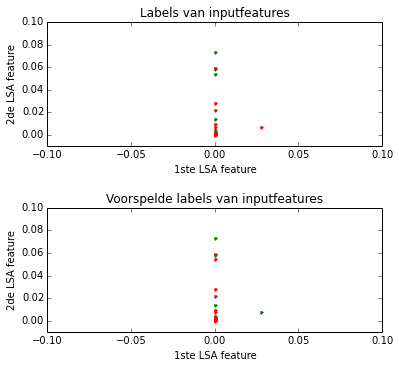
\includegraphics[width=5cm]{resultaten/Trainingsset Boek/Boek/boek-boek-1} }}%
    \subfloat{{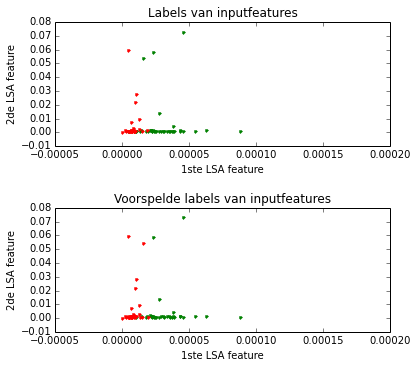
\includegraphics[width=5cm]{resultaten/Trainingsset Boek/Boek/boek-boek-2} }}%
    \subfloat{{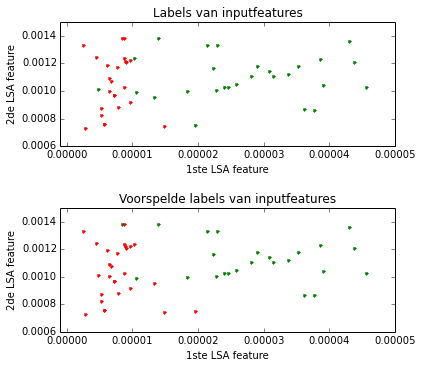
\includegraphics[width=5cm]{resultaten/Trainingsset Boek/Boek/boek-boek-3} }}%
    \caption{Plot van resultaten van de classificatie met een decision Tree, getrained op LSA features met als train- en testset boekrecensies}
    \label{fig:example}%
\end{figure}

